
\section{Design Considerations}

\subsection*{Type of Blockchain}

To satisfy \textbf{NF\_M2} and \textbf{NF\_M1}, we will need to use a public blockchain, which will benefit our project by:

\begin{itemize}
  \item being accessible by a greater amount of people, which should boost availability and scalability (satisfying \textbf{NF\_S1}),
  \item reducing the risk of censorship,
  \item providing greater data integrity (\textbf{NF\_M4})
\end{itemize}

\noindent Ethereum is a public blockchain that allows developers to publish their own distributed applications to it; it comes with an extensive development toolchain so is an obvious choice for this project (\textbf{F\_M8}).


\subsection*{Uploading Content}
\label{subsec:upload-content}

For developers to upload their game (\textbf{F\_M5}), they must provide a digital certificate to prove their identity (\textbf{NF\_M3}) as well as the required metadata (\textbf{F\_M1}) for identifying\footnote{Such as the name, release date, version number, creator and price.}, downloading\footnote{Such as the address of where to purchase the game, the digital certificate of who you're purchasing off and a tracker} and verifying the game\footnote{The root hash and the hashes of each block of data}. The developer is then expected to allow users to purchase the game off them and seed the game to at least an initial group of users.

\begin{figure}[ht]
  \centering
  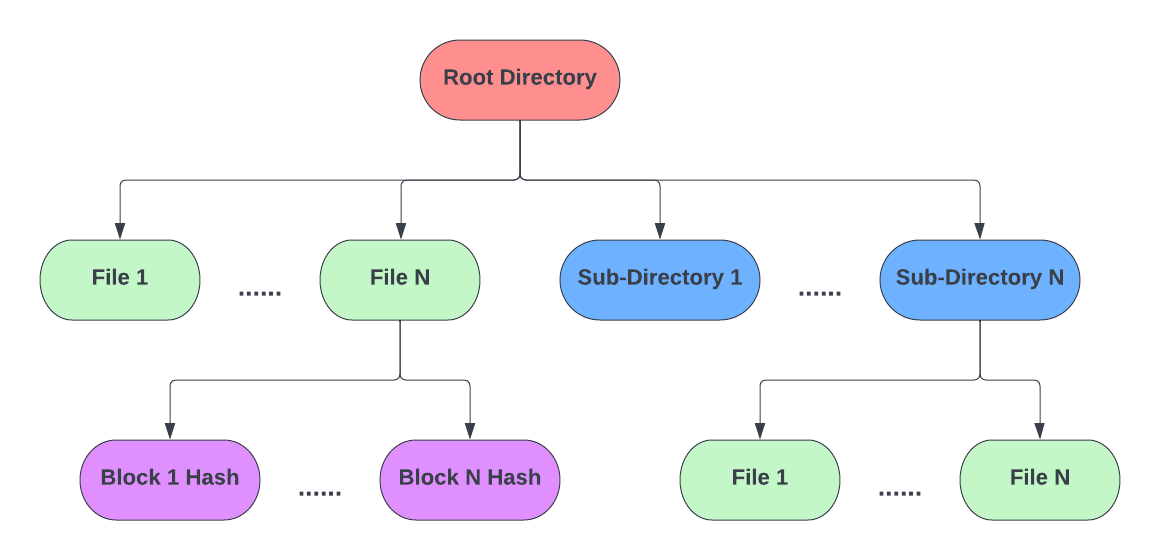
\includegraphics[width=.85\textwidth]{images/diagrams/block-body.png}
  \caption{\textit{How shard data is stored.}}
  \label{fig:hash-storage}
\end{figure}

\subsection*{Purchasing Content}

Users will purchase content from developers using Ether (\textbf{F\_M9}) and will be provided with a proof of purchase (\textbf{F\_M10}) that is encrypted with their private key and can be used by any node in the network to verify the purchase.

\subsection*{Downloading Content}

Games will be content addressable, using their root hash stored on the blockchain, and will allow users to discover nodes to download off of (\textbf{F\_M3}). Once a user finds a node it will:

\begin{enumerate}
  \item Send their proof of purchase of the desired game (\textbf{F\_S2}).
  \item request individual shards from the node using the shard's hash (\textbf{F\_M2}),
  \item use the metadata from the blockchain to verify the block's contents (\textbf{F\_M7}),
  \item send a confirmation message that proves the successful transfer of a block (\textbf{F\_S1}), 
  \item and repeat this until the entirety of the game is installed (\textbf{F\_M6}).
\end{enumerate}

\noindent Shards will be downloaded in a similar order to that of BitTorrent, which is described in Section~\ref{subsec:bittorrent-download}.

\subsection*{Updating Content}

To satisfy \textbf{F\_M4}, developers will perform the same steps as in Section~\ref{subsec:upload-content} but will also include the hash of a previous block that contains the older version of the game. This will include the restriction that only the original uploader can upload an update to a piece of software (\textbf{NF\_S2}).

\begin{figure}[ht]
  \centering
  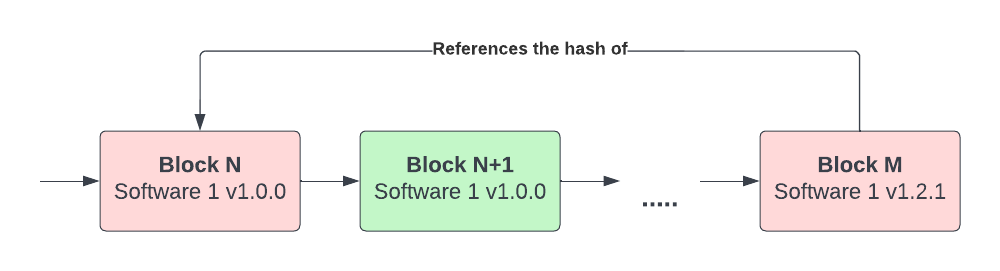
\includegraphics[width=.85\textwidth]{images/diagrams/update-software.png}
  \caption{\textit{How blocks can relate to older blocks.}}
\end{figure}

\noindent It is likely that many shards will persist between versions so a node will only ever download the changed or new data. To satisfy \textbf{F\_C1}, a node may optionally keep older shards that have been removed or changed.


\subsection*{Proving Contribution}

When a user purchases a piece of software they will be granted a unique seeder token. When a user successfully downloads a shard of data off of a peer they will reply with a confirmation message, containing this seeder token, that is encrypted using the developers public key. When a user wants to prove that they have contributed to the distribution of the game, they will send a collection of these messages to the developer, who will judge their validity.

\subsection*{Sequence Diagram}

\begin{figure}[ht]
  \centering
  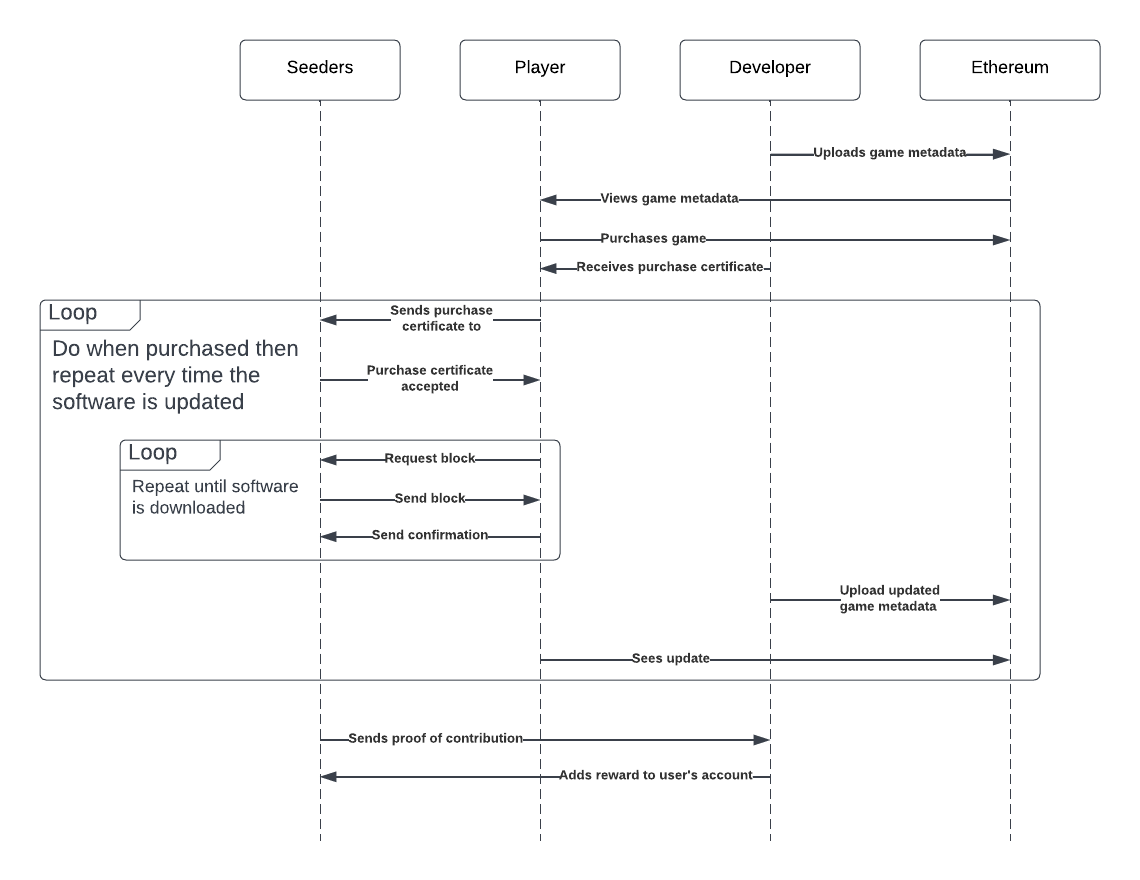
\includegraphics[width=.95\textwidth]{images/diagrams/seqeunce-diagram.png}
  \caption{\textit{The main interactions within the application.}}
\end{figure}